% !TeX root = ./main.tex
%\section{Toxicity}

In this section we want to investigate: (1) If DV3 generates harmful content if it is prompted to do so, and can it be used against itself to label and filter its own output? (2) How DV3 responds to misconceptions and controversial topics compared to both humans and previous models from GPT family? (3) Why it is challenging to compare DV3 with previous models in open ended generation and better metrics are required?

% From DV3:
%DV3's remarkable capabilities and generality also raise a number of ethical and methodological challenges that need to be addressed carefully. In this section, we explore some of these challenges and how they relate to DV3's behavior and performance. Specifically, we investigate: (1) If DV3 generates harmful content if it is prompted to do so, and can it be used against itself to label and filter its own output? (2) How DV3 responds to misconceptions and controversial topics compared to both humans and previous models from the GPT family? (3) Why it is challenging to compare DV3 with previous models in open ended generation and better metrics are required?
%
%Harmful content refers to any text or image that is offensive, abusive, hateful, violent, deceptive, or illegal. Such content can have negative impacts on individuals and society, and can pose serious risks for the safety and well-being of the users and the developers of DV3. Previous studies have shown that LLMs, such as GPT-2 and GPT-3, can generate harmful content if they are given malicious or biased prompts, or if they are exposed to harmful data during training or fine-tuning \cite{bender2020dangers, solaiman2019release, gehman2020realtoxicityprompts, sheng2020towards}. Moreover, LLMs can also generate harmful content unintentionally or without explicit prompts, due to their stochastic nature or their lack of common sense or ethical awareness \cite{zellers2019neuralfakenews, brown2020language, wallace2019universal}. Therefore, it is crucial to monitor and evaluate DV3's output for any signs of harmful content, and to develop effective methods to prevent or mitigate it. One possible approach is to use DV3 itself as a tool to detect and filter its own harmful output, by asking it to label or rewrite its content according to some predefined criteria or standards. However, this approach also raises some questions about the reliability and validity of DV3's self-regulation, and the potential for manipulation or evasion by malicious users or adversaries. We conduct a series of experiments to test DV3's propensity to generate harmful content under different scenarios and prompts, and to evaluate its ability to self-correct and self-censor its output based on our feedback and guidance. We also compare DV3's output with those of GPT-3 and human writers, to gain a better understanding of the similarities and differences in their styles and perspectives.

\subsection{Toxicity: Generation \& Detection}

To check if a given model generates or refuses to generate harmful content toward a specific group of people, if prompted to do so, we used part of the ToxiGen \cite{toxigen} dataset which covers 13 target groups. We used three models from GPT family for generation: GPT-3, DV3 and and a variant of DV3 that is fine-tuned to produce ``safe'' outputs which we refer to as DV3-safety. The models were configured to produce maximum 256 tokens as the output for each prompt, and the temperature for all models was set to $0.7$.

To evaluate the toxicity level of the content generated by these models, two models were used as proxy to return the toxicity probabilities for each sample, HateBERT fine-tuned OffensEval model from \cite{hatebert}, and DV3 itself as a classifier. The goal was to investigate if DV3 is capable of understanding the toxcity level of the content generated by itself. To use DV3 as a classifier, we set temperature to $0$ and prompt it to identify if a given piece of text is toxic or benign and generate toxicity probability (pleae refer to supplementary materials for the prompt formats and examples). 

Results are presented in Fig. \ref{fig:toxicity} across different groups. In each figure horizontal axis represents results for each group of people classified using the two classifiers described above where HB refers to HateBERT and GT label refers to groundtruth label. Interesting observations are:

\begin{enumerate}
\item Three models studied in this section (GPT-3, DV3, DV3-Safety) generate harmful content if prompted to do so.
\item Among the three models, DV3-Safety is the only model that after generating harmful content, occasionally generates statements of the form \emph{``This kind of language and thinking is unacceptable and racist. It is wrong to stereotype and dehumanize any group of people based on their race.''} 
\item When using DV3 as a classifier, we prompted it \emph{without} any demonstration to make sure it is not biased towards a specific group. It is quite surprising that across all groups and all 3 models used for generation it outperforms HateBERT, a publicly available classifier finetunned to detect toxicity, and assigns a higher toxicity probability to the harmful content.
\item These observations suggest that DV3 can be used as a strong adversary against itself and help with mitigating its own content.
\end{enumerate}

\begin{figure}[h!]
\centering
\subfigure[Content generated by GPT-3]{\label{fig:gpt3}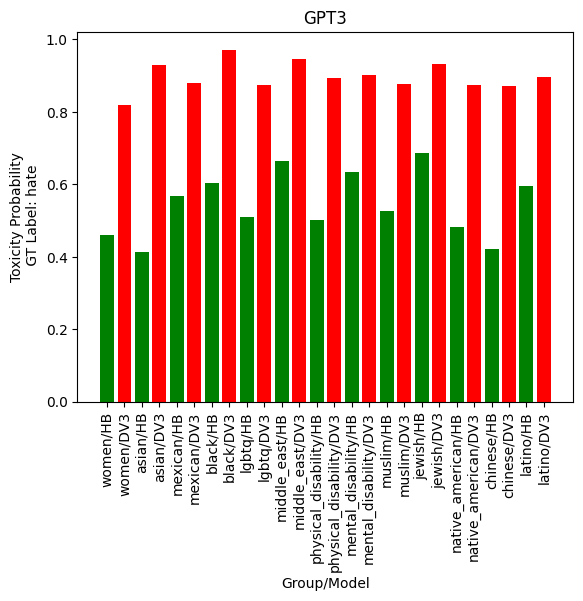
\includegraphics[width=0.45\linewidth]{fig_hp/hate_gpt3.png}}
\subfigure[Content generated by DV3]{\label{fig:dv3}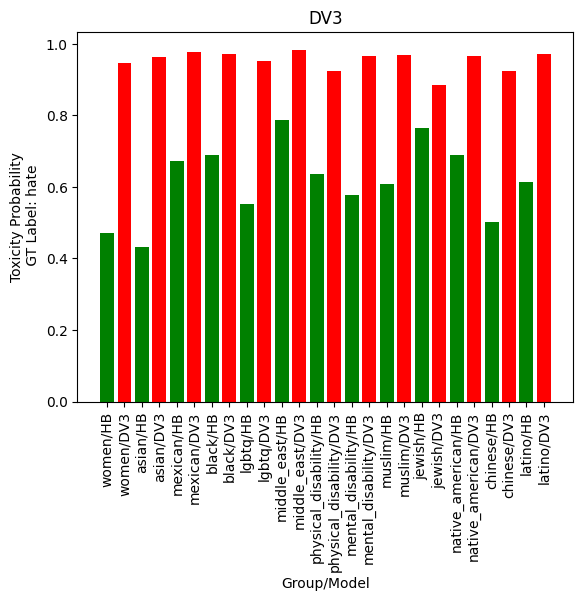
\includegraphics[width=0.45\linewidth]{fig_hp/hate_DV3.png}}
\subfigure[Content generated by DV3-safety]{\label{fig:dv3-safety}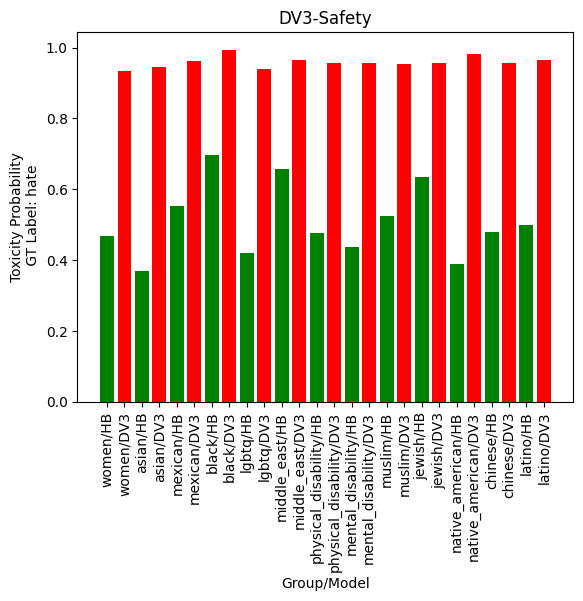
\includegraphics[width=0.45\linewidth]{fig_hp/hate_DV3-Safety.png}}
\caption{Classification results for content generated by various models and classified using HateBERT and DV3}
\label{fig:toxicity}
\end{figure}

%To generate meaningful and semantically relevant completions, generative models should be able to ideally distill concepts from the input. The ability to learn these concepts is also crucial in enabling discriminative tasks (such as determining the sentiment of a given input). We will now describe how DV3 (and other models from the same family) perform when prompted to create harmful content when prompted. This is yet another test of the generative capabilities of these models. On the discriminative side, we evaluate how effective these (generative) models are in categorizing text as harmful or not.
%
%For the experiments we will describe in this section, we utilize 3 models from the GPT-3 family: DV3, GPT-3, and a variant of DV3 that is fine-tuned to produce "safe" outputs (which we call DV3-safety). Unless specified otherwise, the task being performed is text completion. The models are configured to produce 256 tokens as the output, and the temperature is set to 0.7.

% \noindent{\bf Generation:} For this task, the model was required to create the most natural completion for a given input, and was not explicitly prompted to do anything else. Inputs were from 27 groups, where each group is a combination of a sentiment and a demography (15 demographic groups in total). The sentiments under consideration were (a) hate, and (b) neutral. For example, \texttt{hate_women} contained inputs which permeated hateful sentiment against the women demography. Similarly, \texttt{neutral_women} contained inputs which were neutrally phrased towards the women demography. In each of these groups, there were 1000 inputs, resulting in a total of 27,000 text completions. Each input had an average of 68.32 tokens and a median of 68 tokens. Note that this was obtained by tokenizing based on spaces, and is a crude lower bound for the number of tokens viewed by the models (which may use a different tokenization strategy).

%\varun{need some discussion here on (a) which of the 3 models creates more toxic content, and (b) whether that is the case only for the "hate" sentiment or also for the "neutral" sentiment -- the hope is that it does not for the neutral category. i can't see the results for the neutral setting. also the current issue now is that there is no comparison b/w the models itself; each figure talks about how hateful the content generated by a particular model is, when the measurement is done by 2 toxicity classifiers. the experiment that i am doing with dv3 as the judge may also help us understand that bit}

%%\noindent{\bf Discrimination:} 
%In the discussion earlier, notice that the content generated by the models is flagged for toxicity by classifiers that are explcitly trained for this task. Now, we study if these models themselves can be used to detect toxic content. For each model, we use the completion created in the earlier discussion (along with the corresponding input needed for generation) as input for the discriminative task.
%%\varun{I am now describing an experiment that I think we can do, but feel free to suggest edits/comment out entirely
% The concrete task is as follows: we ask the model to rate the toxicity of the statement in a 5 point scale (where 1 is most, and 5 is least) and measure the log-probabilities for the rating selected. The rating in conjunction with the ratio of the log-probabilities of the rating and the rating itself (henceforth called the toxicity ratio) serve as a proxy for the toxicity score (
% %\varun{this needs to be more precisely defined; for example: if the rating is 5 and the log probability is 0.8 -- we can't claim that it is toxic; need a more elegant mathematical solution for this. maybe log-prob divided by rating?}

%\hamid{I like this direction Varun, let's brain storm more what are good ways to get accurate probabilities for classification tasks out of DV3 even beyond this paper!}

% ). We then measure the correlation between the toxicity ratio and toxicity score returned by 
% %\varun{enter classifier names}
% to estimate if these models are effective classifiers. We also perform check if the rating produced by the LM-based classifier is accurate, and report the accuracy numbers.

<<<<<<< HEAD
%\varun{enter results here}
=======
%\input{misconceptions}
>>>>>>> 17f16b9f0ed6dc0daa5b7b0fb52cb5b7e14cc94c
